\documentclass{beamer}

\usetheme{default}
\beamertemplatenavigationsymbolsempty

\definecolor{fore}{RGB}{249,242,215}
%{249,242,215}
\definecolor{back}{RGB}{51,51,51}
%{RGB}{51,51,51}
\definecolor{title}{RGB}{230,96,6}
%{255,0,90}
%http://meyerweb.com/eric/tools/color-blend/
%http://mikedewar.wordpress.com/2009/02/25/latex-beamer-python-beauty/
%http://www.census.gov/population/international/data/worldpop/table_population.php

\setbeamercolor{titlelike}{fg=title}
\setbeamercolor{normal text}{fg=fore,bg=back}

\usepackage{caption}
\usepackage{listings,bera}
\definecolor{keywords}{RGB}{255,102,0}
%{255,0,90}
\definecolor{comments}{RGB}{51,153,204}
\setbeamertemplate{caption}[numbered]
\lstset{language=Python,
keywordstyle=\color{keywords},
commentstyle=\color{comments}\emph}


\begin{document}

%\begin{frame}[fragile]
%\frametitle{Generic slide}
%\begin{itemize}
%\item thing 1  
%\item thing 2 
%\item thing 3 
%\item thing 4
%\end{itemize} 
%\end{frame}

\begin{frame}[fragile]
\frametitle{Python for Ecologists}
\begin{itemize}
  \item Assuming not much programming experience
  \item Immersion approach 
\begin{itemize}
  \item Short lecture on Python topic
  \item Hands-on Python exercises 
  \item Rinse \& repeat
\end{itemize}
  \item Will use ecological examples as much as possible
\end{itemize} 
\end{frame}

\begin{frame}[fragile]
\frametitle{Your presenters}
\begin{itemize}
\item Tom Purucker  
\item Tao Hong 
\item Chance Pascale
\end{itemize} 
\end{frame}

\begin{frame}[fragile]
\frametitle{Why bother with Python when I have R?}
\begin{itemize}
\item A scripting language (like R) but also, 
\item A high level programming language
\item Designed to produce readable code 
\item Cross-platform 
\end{itemize} 
\end{frame}

\begin{frame}[fragile]
\frametitle{\"{u}bertool Python project}
\begin{itemize}
  \item{http://www.ubertool.org}
  \item{Created with Python as the science engine}
  \item{Integrates easily with web technologies such as HTML, JavaScript, JQuery}
\end{itemize} 
\begin{figure}
 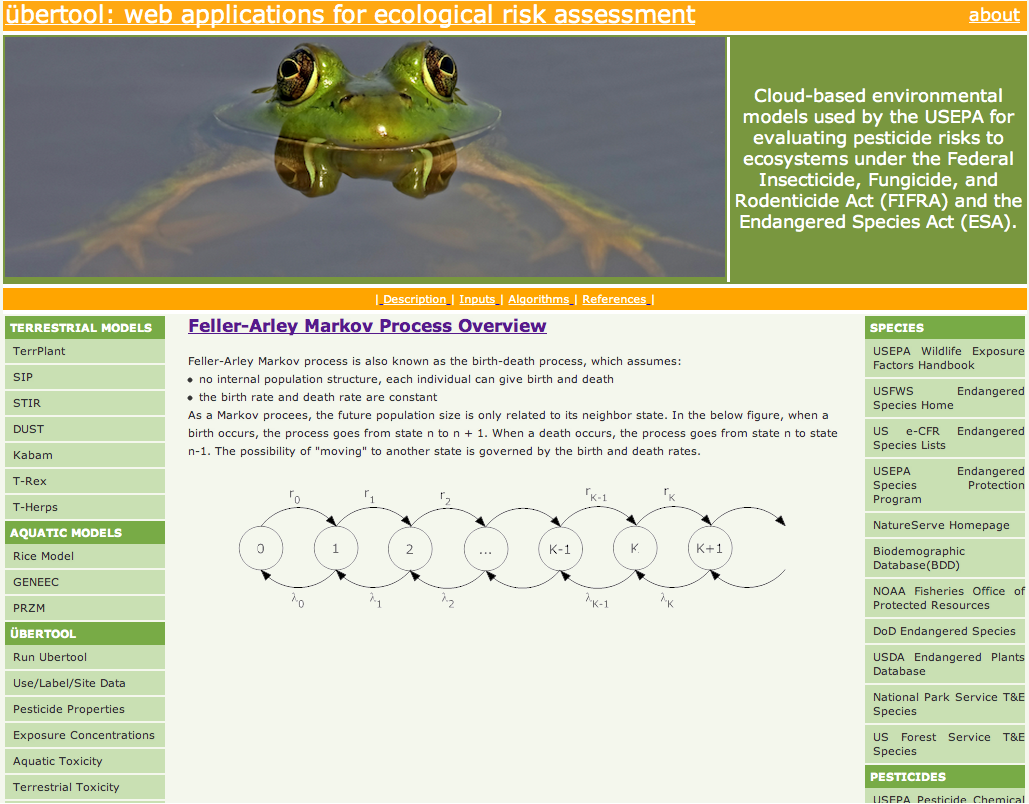
\includegraphics[scale=0.18]{ubertool.png} 
 \caption{\"{u}bertool ecological risk web application}
\end{figure}
\end{frame}

\begin{frame}[fragile]
\frametitle{Getting setup}
\begin{itemize}
  \item{We will use Python 2.7 (not 3)}
  \item{http://www.python.org/getit/}
  \item{For Windows users: http://portablepython.com/wiki/Download}
\end{itemize} 
\end{frame}

\begin{frame}[fragile]
\frametitle{Some extra libraries to install}
\begin{itemize}
  \item{numpy- http://sourceforge.net/projects/numpy/}
  \item{scipy- http://sourceforge.net/projects/scipy/files/}
\end{itemize} 
\end{frame}

\begin{frame}[fragile]
\frametitle{Need a text editor}
\begin{itemize}
  \item{Linux-/}
  \item{Mac- TextWrangler, Smultron, TextEdit (already installed)}
  \item{Windows- Notepad (already installed), Notepad++, TextPad}
\end{itemize} 
\end{frame}

\begin{frame}[fragile]
\frametitle{Python IDLE IDE}
\begin{itemize}
  \item{http://www.ubertool.org}
  \item{Created with Python as the science engine}
\end{itemize} 
\end{frame}

\begin{frame}[fragile]
\frametitle{Python objects}
\begin{itemize}
\item Everything in Python is an object with these properties
\begin{itemize}  
  \item an identity (id) 
  \item a type (type)
  \item a value (mutable or immutable)
\end{itemize}
\end{itemize} 
\end{frame}

\begin{frame}[fragile]
\frametitle{Each Python object has an id}
\begin{lstlisting}
>>> n_predators = 12
>>> id(n_predators)
4298191056
\end{lstlisting} 
\end{frame}

\begin{frame}[fragile]
\frametitle{Each Python object has a type}
\begin{lstlisting}
>>> n_predators = 12
>>> type(n_predators)
<type 'int'>
\end{lstlisting}
\end{frame}

\begin{frame}[fragile]
\frametitle{Each Python object has a value}
\begin{itemize}
\item String, integer, and tuple object values are \emph{immutable}
\begin{lstlisting}
>>> n_prey = 88
>>> id(n_prey)
4298193184
>>> n_prey = 96
>>> id(n_prey)
4298192992 # id for n_prey has changed
\end{lstlisting}
\item Dictionary and list items are \emph{mutable}
\begin{lstlisting}
>>> birds = ["cardinal", "oriole"]
>>> id(birds)
4332756000
>>> birds.append("gnatcatcher")
>>> id(birds)
4332756000 # id is still the same
\end{lstlisting}
\end{itemize}
\end{frame}

\begin{frame}[fragile]
\frametitle{Variables}
\begin{lstlisting}
pop_size = 112 # integer
pop_density2 = 4 # still an integer
pop_density = 4. # float
species_name = "Oedipina complex" # string
species_name = "4" # still a string
\end{lstlisting}
\end{frame}

\begin{frame}[fragile]
\frametitle{Python variable naming conventions}
\begin{itemize}
\item all lowercase
\item cannot start with numbers
\item separate\_words\_with\_underscores
\item Style Guide for Python: 
\begin{itemize}
\item http://www.python.org/dev/peps/pep-0008/
\end{itemize}
\end{itemize}
\end{frame}

\begin{frame}[fragile]
\frametitle{Exercise 1}
\begin{lstlisting}
variables.py
\end{lstlisting}
\end{frame}

\begin{frame}[fragile]
\frametitle{Hello world! (from an interpreter)}
\begin{lstlisting}
>>> python
>>> print "Hello world!"
Hello world!
\end{lstlisting}
\end{frame}

\begin{frame}[fragile]
\frametitle{Hello world! (from a script)}
\begin{lstlisting}
# save this in a text file as hello.py
print "Hello world!"
# then run at the command prompt with 'python hello.py'
\end{lstlisting}
\end{frame}

\begin{frame}[fragile]
\frametitle{Hello world! (as an executable)}
\begin{lstlisting}
#!/usr/bin/env python
# the above line automatically invokes Python
# save this in a text file as hello_exe.py
print "Hello world!"
# we can run this with simply "hello"
\end{lstlisting}
\end{frame}

\end{document}